\documentclass[a4paper]{article}
\usepackage[letterpaper, margin=1in]{geometry} % page format
\usepackage{listings} % this package is for including code
\usepackage{graphicx} % this package is for including figures
\usepackage{amsmath}  % this package is for math and matrices
\usepackage{amsfonts} % this package is for math fonts
\usepackage{tikz} % for drawings
\usepackage{hyperref} % for urls
\usepackage{amsmath} %for math
\usepackage[shortlabels]{enumitem} % for the cool itemize letters
\usepackage{graphicx}
\usepackage{calligra}

\DeclareMathOperator*{\argmin}{\arg\min}

\title{Homework 0}
\author{Amy Pitts}
\date{1/23/19}

\begin{document}
\lstset{language=Python}

\maketitle

\section{Instructions}
\textit{No deliverables}

\section{Course Setup}

\subsection{Python}
After downloading all the required packages running
this script shows that everything is install and 
their versions. 
%proof that the intalls worked
\lstinputlisting[language=Python,frame=single]{install_check.py}
Output of the script file  \\
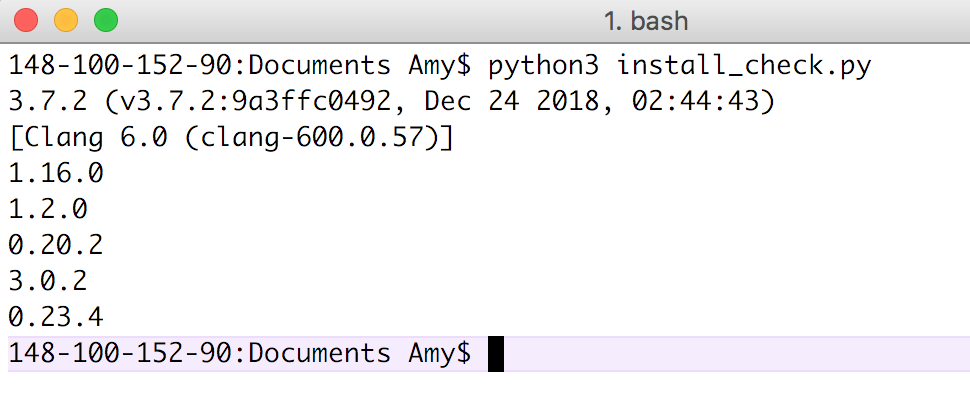
\includegraphics{python_downloads}

\subsection{GitHub Class Repository}

- Github name and class repository: \\

\includegraphics{github_name}\\
\bigskip
- Link to class repository: \textit{https://github.com/amypitts01/data440/invitations} \\
\bigskip
- Proof that pablorp80 was asked to be a collaborator: \\

\includegraphics[width=1\textwidth]{proof_of_collab}


\subsection{Kaggle Account}
My Kaggle user name is: \textbf{Amypitts01} \\

\includegraphics[width=.9\textwidth]{kaggle_proof}

\section{Mathematics Requirements}
\textit{No deliverables}

\section{Problems}

%-------------------QUESTION 1----------------------
%---------------------------------------------------
1. For the function $g(x) = -3x^2+24x-30$, find the value for x
that maximizes $g(x)$.  
\smallskip
\\
\indent \textbf{Solution:} To maximize this function the first step
is to take the derivative such that $g'(x) = -6x+24$. Setting
the derivative equal to 0 to find the critical values we have:
\begin{align*}
-6x+24&=0 \\
-6(x-4)&=0\\
x-4&=0\\
x=4.
\end{align*}
The maximun occurs when the derivative is positive left of the
critical value and negative right of the critical value. Since
there is only one critical value we do not need to compare to 
other critical values to find the biggest $y$ value.
To show that $4$ is in fact a max we see that:\\
\indent Left: $g'(0)=-6(0)+24=24$ \textit{positive} \\
\indent Right: $g'(10)=-6(10)+24=-36$ \textit{negative} \\
Therefore, $x=4$ maximizes the function.
\\
\\
%-------------------QUESTION 2----------------------
%---------------------------------------------------
2. Consider the following function:
\begin{equation*}
f(x)=3x_0^3-2x_0x_1^2+4x_1-8
\end{equation*}
what are the partial derivatives of $f(x)$ with respect to $x_0$ and $x_1$.
\\
\textbf{Solution:}
\\
\begin{align*}
\frac{\partial f}{\partial x_0}&= 9x^2_0-2x_1^2 \\
\frac{\partial f}{\partial x_1}&= -4x_0x_1+4
\end{align*}
\\
\\
%-------------------QUESTION 3----------------------
%---------------------------------------------------
3. Consider the matrix
$ A=\left[\begin{matrix}
1 & 4 & -3 \\
2 & -1 & 3
\end{matrix}\right] $ and
$ B=\left[\begin{matrix}
-2 & 0 & 5 \\
0 & -1 & 4
\end{matrix}\right] $m then answer the following and verify your answers in Python:
\begin{enumerate}[(a)] % (a), (b), (c), ...
\item can you multiply the two matrices? ellaborate on your answer.
\begin{itemize}
  \item \textbf{Solution:} No you can not multiply the two
  becuase $A$ does not have the same number of collumns and
  $B$'s rows. They are both $(2,3)$ matrices and to
  be able to multiply $A$ would need to be $(2,3)$ and $B$ dims $(3,2)$
  or $A$ could be $(3,2)$ and $B$ $(2,3)$.
\end{itemize}
\item multiply $A^T$ and $B$ and give its \textit{rank}.
\begin{itemize}
  \item \textbf{Solution:} First we need to find the transopes
  of $A$. This results in $A^T = \left[\begin{matrix}
    1 & 2   \\
    4 & -1  \\
    -3 & 3
  \end{matrix}\right] $. Now we can multiply $A^TB$. This gives us
  $A^TB = \left[\begin{matrix} 1 & 2 \\ 4 & -1 \\-3 & 3 \end{matrix}\right]
  \left[\begin{matrix}  -2 & 0 & 5 \\ 0 & -1 & 4 \end{matrix}\right] \\=
    \left[\begin{matrix}
      (1)(-2)+(2)(0) & (1)(0)+(2)(-1) & (1)(5)+(2)(4) \\
      (4)(-2)+(-1)(0) & (4)(0)+(-1)(-1) & (4)(5)+(-1)(4) \\
      (-3)(-2)+(3)(0) & (-3)(0)+(3)(-1) & (-3)(5)+(3)(4)
    \end{matrix}\right] \\
    = \left[\begin{matrix}
      -2 & -2 & 13 \\
      -8 & 1 & 16 \\
      6 & -3 & -3
    \end{matrix}\right]
    $.
  \item \textbf{Solution:} Next to find the rank we need to
  row reduce until we reach row echelon form. Then we have
  $ \left[\begin{matrix}
    -2 & -2 & 13 \\
    -8 & 1 & 16 \\
    6 & -3 & -3
  \end{matrix}\right] \rightarrow
  \left[\begin{matrix}
    1 & 1 & \frac{-13}{2} \\
    -8 & 1 & 16 \\
    6 & -3 & -3
  \end{matrix}\right] \rightarrow
  \left[\begin{matrix}
    1 & 1 & \frac{-13}{2} \\
    0 & 9 & -36 \\
    0 & -9 & 36
  \end{matrix}\right] \rightarrow
  \left[\begin{matrix}
    1 & 1 & \frac{-13}{2} \\
    0 & 1 & -4 \\
    0 & 0 & 0
  \end{matrix}\right]
  $.
  The row eachelon of $A^TB$ shows two independent row vectors
  therefore the \textbf{rank is 2}.
\end{itemize}
\item (extra credit) let $c=\left[\begin{matrix} 1 & 0  \\ 0 & 2
  \end{matrix}\right] $ be a new matrix; what is the result of $AB^T+C^{-1}$?
  \begin{itemize}
    \item \textbf{Solution:} First we need to find $c^{-1}$. This gives us \\
    $c^{-1} = \frac{1}{ad-bc} 
      \left[\begin{matrix} d & -b \\ -c & a \end{matrix}\right] 
      = \frac{1}{2} \left[\begin{matrix} 2 & 0 \\ 0 & 1 \end{matrix}\right]
      =  \left[\begin{matrix} 1 & 0 \\0 & \frac{1}{2} \end{matrix}\right]$. \\
    Now we need to find $B^T$. Then we have 
    $B^T = \left[\begin{matrix}-2 & 0 \\0 & -1 \\4 & 5 \end{matrix}\right]$. 
    Now we can find $AB^T$. Thus we have
    $AB^T = \left[\begin{matrix}1 & 4 & -3 \\2 & -1 & 3\end{matrix}\right] 
      \left[\begin{matrix} -2 & 0  \\0 & -1 \\ 4 & 5 \end{matrix}\right] 
      = \left[\begin{matrix} -14 & -19  \\8 & 16 \end{matrix}\right]$. 
    Then adding in $C^{-1}$ we get \\
    $AB^T+C^{-1} = \left[\begin{matrix} -14 & -19 \\8 & 16 \end{matrix}\right] 
      + \left[\begin{matrix} 2 & 0  \\0 & \frac{1}{2} \end{matrix}\right] 
      = \left[\begin{matrix} -13 & -19  \\ 8 & 16.5 \end{matrix}\right].$
  \end{itemize}
\end{enumerate}

\indent \textbf{Solution:}
Here is the scipt I ran to check the matrices. 
\lstinputlisting[language=Python,frame=single]{matrix_checks.py}
Python answer for 3.a \\
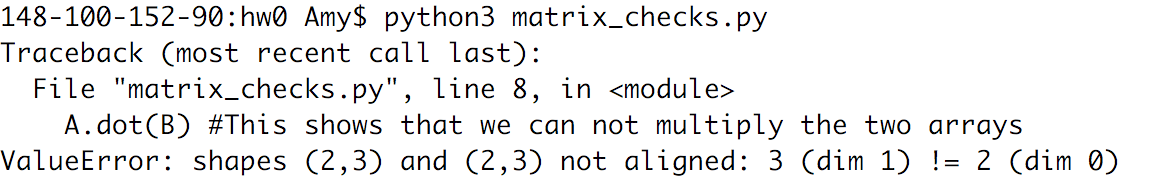
\includegraphics[width=1\textwidth]{matrix_errors} 
\smallskip \\
Python answer for 3.b \\
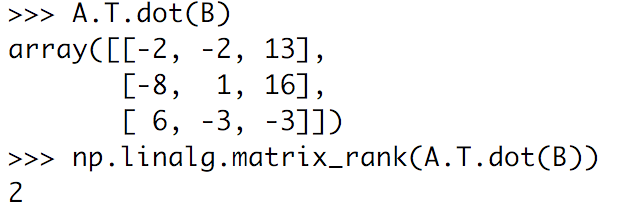
\includegraphics[width=.6\textwidth]{matrix_answers}
\\
%-------------------QUESTION 4----------------------
%---------------------------------------------------
4. Give the mathematical definitions of the simple Gaussian,
multivariate Gaussian, Bernoulli, binomial, and exponential distributions.
\\
\indent \textbf{Solutions:}
\smallskip
\\
\indent \textbf{Gaussian:} This is also known as the normal distibution
and has a pdf of $f_X(x) = \frac{1}{\sigma \sqrt{2\pi}}exp\{- \frac{(x-\mu)^2}{2\sigma^2} \}$
and it is notation is $N(\mu,\sigma^2)$.
\smallskip
\\
\indent \textbf{Multivariate Gaussian:} This distrabution has
a pdf of $f_X(x)=(2\pi)^\frac{k}{\Sigma} |\Sigma|^{\frac{-1}{2}} e^{\frac{-1}{2}(x-\mu)^T\Sigma^{-1}(x-\mu)}$
and it is notation is MVN$(\mu,\Sigma)$.
\smallskip
\\
\indent \textbf{Bernoulli:} This distrabution has a pdf of
$f_X(x) = p^x(1-p)^{1-x}$ with notation Bern$(p)$.
\smallskip
\\
\indent \textbf{binomial:} This distrabution has a pdf of
$f_X(x)= \binom{n}{k} p^x(1-p)^{n-x}$ with notation Bin$(n,p)$.
\smallskip
\\
\indent \textbf{exponential distributions:} This distrabution has a pdf of
$f(x;\lambda)= \begin{cases} \lambda e^{-\lambda x} & x\geq0 \\ 0 & x<0 \end{cases}$.
\bigskip
\\
%-------------------QUESTION 5----------------------
%---------------------------------------------------
5. (extra credit) What is the relationship between the Bernoulli
and binomial.
\\
\indent \textbf{Solution:} The Bernoulli distributions is made up of Bernoulli
trails where an even occurs $p$ or the even does not occur $1-p$.
There is only two options success or failure. When you have $n$
independent Bernoulli trails those successes and failures are
represented in a Binomial Distribution.
%https://www.unf.edu/~cwinton/html/cop4300/s09/class.notes/DiscreteDist.pdf
\\
\\
%-------------------QUESTION 6----------------------
%---------------------------------------------------
6. Suppoe that random variable $X \sim N(2,3)$. What is its expected
value?
\\
\indent \textbf{Solution:} $ N(2,3)$ is a normal distrabution it has a
$E[x]=\mu$. Since $N(\mu,\sigma^2)$ we have that in our case $E[x]=2$.
\\
\\
%-------------------QUESTION 7----------------------
%---------------------------------------------------
7. An \textit{euclidean projection} of a $d$-dimensional point
$y\in \mathbb{R}^d$ to a set $\mathcal{Z}$ is given by the following
optimzation problem:
\begin{center}
$x^*=\argmin_x ||x-y||^2_2$, subject to $x\in \mathcal{Z}$
\end{center}
where $\mathcal{Z}$ is the feasible set, $||\cdot||_2$ is the
\textit{l}$_2$-norm (euclidean) of a vector, and $x^*\in\mathbb{R}^d$
is the projected vector.
\begin{enumerate}[(a)]
\item What is $x^*$ if $y=1.1$ and $\mathcal{Z}=\mathbb{N}$?
  \begin{itemize}
    \item \textbf{Solution:} the $\argmin_x ||x-y||^2_2$ is the 
    value of $x$ for which $||x-y||^2_2$ attains it's min value.
    Since $x \in \mathcal{Z} = \mathbb{N}$ we can use trial and errors
    to find the min. \\ 
    First lets start with $x=0$ then we have:
    $||0-1.1||^2_2 = \sqrt{(0-1.1)\cdot (0-1.1)}^2=1.21$. \\ 
    Now looking at $x=1$ we have: $||1-1.1||^2_2 = \sqrt{(1-1.1)\cdot (1-1.1)}^2 =0.01$. \\
    Finally looking at $x=2$ we have $||2-1.1||^2_2 = \sqrt{(2-1.1)\cdot (2-1.1)}^2= .81$. \\
    Because the natural numbers only increase from here the smallest
    value is going to be made when $x=1$ obtaining a $x^*=0.01$. 
  \end{itemize}
\item Locate $x^*$ in the following picture:\\
The red dot should be the closest point on the 
perimeter of the $\mathcal{Z}$. \\
  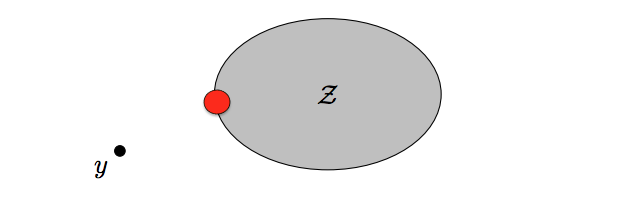
\includegraphics[width=.5\textwidth]{pic_7_answer.png} \\

\end{enumerate}
\textbf{Solution:}
\\
\\
%-------------------QUESTION 8----------------------
%---------------------------------------------------
8. Suppose that random variable $Y$ has distribution:
\begin{center}
$p(Y=y)=\begin{cases}
e^{-y} & y\ge 0\\
0 & otherwise
\end{cases}$
\end{center}
\begin{enumerate}[(a)]
\item Verify that $\int_{y=-\infty}^{\infty} p(Y=y) dy=1 $
\item What is $\mu_y = E[Y]= \int_{y=-\infty}^{\infty} p(Y=y)ydy$; that is, the expected value of $Y$?
\item What is $\sigma^2=Var[Y]=\int_{y=-\infty}^{\infty} p(Y=y)(y-\mu_y)^2dy$; that is, the variance of $Y$?
\item What is $E[Y|Y\geq 10]$; that is, the expected value of $Y$, given that (or conditioned on) $Y \geq 10$?
\end{enumerate}

\textbf{8.a Solution:}
\begin{align*}
\int_{y=-\infty}^{\infty} p(Y=y) dy &= 1 \\
\int_{-\infty}^{0} 0 dy + \int_{0}^{\infty} e^{-y} dy &= 1 \\
0 - e^{-y} |^{\infty}_0  &= 1 \\
1  &= 1.
\end{align*}

\textbf{8.b Solution:}
\begin{align*}
\mu_y = E[Y] &= \int_{y=-\infty}^{\infty} p(Y=y)y dy \\
&= \int_{-\infty}^{0} 0 dy + \int_{0}^{\infty} ye^{-y} dy \\
&= 0+\int_{0}^{\infty} ye^{-y} dy
\end{align*}
Now we need to do integration by parts. Using $u=y$,
$du=1dy$, $v=-e^{-y}$ and $dv=e^{-y}$ we have:
\begin{align*}
 \mu_y&= \int_{0}^{\infty} ye^{-y} dy \\
 &= -ye^{-y}|_{0}^{\infty} + \int_{0}^{\infty} e^{-y} dy \\
 &= 0 -e^{-y}|_{0}^{\infty} \\
 &= 1.
\end{align*}

\textbf{8.c Solution:}
\begin{align*}
\sigma^2=Var[Y]&=\int_{y=-\infty}^{\infty} p(Y=y)(y-\mu_y)^2dy \\
&=\int_{-\infty}^{0} 0(y-\mu_y)^2dy + \int_{0}^{\infty} e^{-y}(y-\mu_y)^2dy\\
&= \int_{0}^{\infty} e^{-y}(y^2-2y\mu_y+\mu_y^2)dy\\
&= \int_{0}^{\infty} e^{-y}y^2 dy -\int_{0}^{\infty}2e^{-y}y\mu_y dy+\int_{0}^{\infty}e^{-y}\mu_y^2dy
\end{align*}
Now looking at each integral individually we have
\begin{align*}
\int_{0}^{\infty} e^{-y}y^2 dy &= -y^2e^{-y}|_{0}^{\infty} - 2\int_{0}^{\infty} e^{-y}y dy\\
&= 0 +2E[Y] \\
&=  2.
\end{align*}

\begin{align*}
-\int_{0}^{\infty}2e^{-y}y\mu_y dy &= -\int_{0}^{\infty}2e^{-y}y\mu_y dy\\
&= -2\mu_y\int_{0}^{\infty}e^{-y}y dy\\
&= -2\mu_yE[Y]\\
&= -2\mu_y.
\end{align*}

\begin{align*}
\int_{0}^{\infty}e^{-y}\mu_y^2dy = \mu_y^2\int_{0}^{\infty}e^{-y}dy = \mu_y^2.
\end{align*}
Putting this all together we have that
\begin{align*}
Var[Y]= \int_{0}^{\infty} e^{-y}y^2 dy -\int_{0}^{\infty}2e^{-y}y\mu_y dy+\int_{0}^{\infty}e^{-y}\mu_y^2dy
= 2 -2\mu_y+\mu_y^2.
\end{align*}


\textbf{8.d Solution:}
\begin{align*}
E[Y|Y\geq 10] &= \int_{10}^{\infty} p(Y=y)y dy \\
&= \int_{10}^{\infty} ye^{-y} dy
\end{align*}
Now we need to do integration by parts. Using $u=y$,
$du=1dy$, $v=-e^{-y}$ and $dv=e^{-y}$ we have:
\begin{align*}
\int_{10}^{\infty} ye^{-y} dy
 &= -ye^{-y}|_{10}^{\infty} + \int_{10}^{\infty} e^{-y} dy \\
 &= 0 +10e^{-10}-e^{-y}|_{10}^{\infty} \\
 &= 10e^{-10}+e^{-10} \\
 &= 11e^{-10}.
\end{align*}



\end{document}




